\section{基于DTFT的系统频域分析}

本节在频域角度,讨论离散系统的响应。

本节要点:
\begin{itemize}
    \item 离散系统频率响应的概念;
    \item 了解采样频率对输出的影响。
\end{itemize}

%============================================================
\subsection{离散系统的频域响应定理}

\begin{theorem}[离散系统的频域响应定理]
如果一个零状态LTI系统满足绝对稳定的条件,即$\sum_{n=-\infty}^{+\infty}{\left| h\left[ n \right] \right|}<\infty $,则系统对于任意非周期信号$x\left[ n \right] $在时域的输出可以表示为卷积:
\[
y\left[ n \right] =x\left[ n \right] \ast h\left[ n \right]
\]
在频域的输出可以表示为DTFT的乘积:
\[
Y\left( \varOmega \right) =X\left( \varOmega \right) \cdot H\left( \varOmega \right)
\]
\begin{itemize}
    \item $x\left[ n \right] ,y\left[ n \right] $:输入输出信号的时域表达式;
    \item $h\left[ n \right] $:系统的冲激响应;
    \item $X\left( \varOmega \right) ,Y\left( \varOmega \right) $:输入输出信号的DTFT;
    \item $H\left( \varOmega \right) $:{\bf 离散系统的频率响应函数}(frequency response function),或称{\bf 系统函数}(system function),即$h\left[ n \right] $的傅里叶变换。
\end{itemize}
\end{theorem}

一个满足绝对稳定条件的LTI系统对任何输入的信号,系统会单独作用其各个频率分量的幅度和相位:
\begin{align*}
&\left| Y\left( \varOmega \right) \right|=\left| X\left( \varOmega \right) \right|\cdot \left| H\left( \varOmega \right) \right| \\
&\angle Y\left( \varOmega \right) =\angle X\left( \varOmega \right) +\angle H\left( \varOmega \right)
\end{align*}

%============================================================
\subsection{理想低通和采样频率对信号的影响}

数字系统对时域信号通常的做法是先采样进行离散化,再通过一个数字滤波器。
这里考察数字滤波器(即系统本身)和采样过程对信号通过性的影响。

首先考察滤波器对信号的输出结果。
由于DTFT的周期性,离散系统的频率响应函数是一个$T=2\pi $的周期函数。
假设一LTI离散系统(理想低通)有如下频率响应函数:
\begin{figure}[ht]
\centering
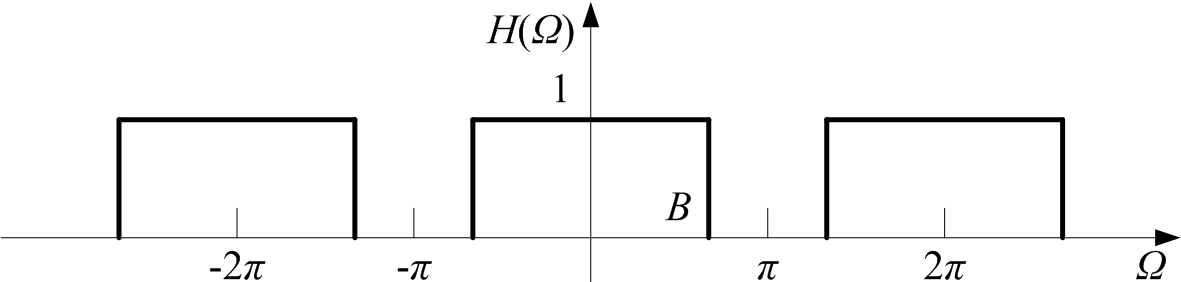
\includegraphics[height=2.5cm]{6.2.2-1.png}
\end{figure}
\[
H\left( \varOmega \right) =\sum_{n=-\infty}^{+\infty}{p_{2B}\left( \varOmega +2\pi n \right)}
\]

对比CTFT的系统频域分析,这里要注意几点:
\begin{itemize}
    \item 由于DTFT的周期性,一般考察区间$\left[ -\pi ,\pi \right] $,往0方向的是低频,往$\pm \pi $方向的是高频。
    \item 由于的频谱的对称性,考察区间可缩小为$\left[ 0,\pi \right] $。
\end{itemize}

\begin{tcolorbox}
这样的理想低通是不存在的,因为其冲激响应$h\left[ n \right] =\frac{B}{\pi}\sin\mathrm{c}\left( \frac{B}{\pi}n \right) $不符合因果性。
\end{tcolorbox}

对于简单的正弦信号$x\left[ n \right] =A\cos \left( \varOmega _0n \right) $,其DTFT有
\[
X\left( \varOmega \right) =\sum_{m=-\infty}^{\infty}{A\pi \left[ \delta \left( \varOmega +\varOmega \,\,_0+2\pi m \right) +\delta \left( \varOmega -\varOmega \,\,_0+2\pi m \right) \right]}
\]
只要$\varOmega _0\leqslant B$,信号就能通过该系统,如下图。
\begin{figure}[h]
\centering
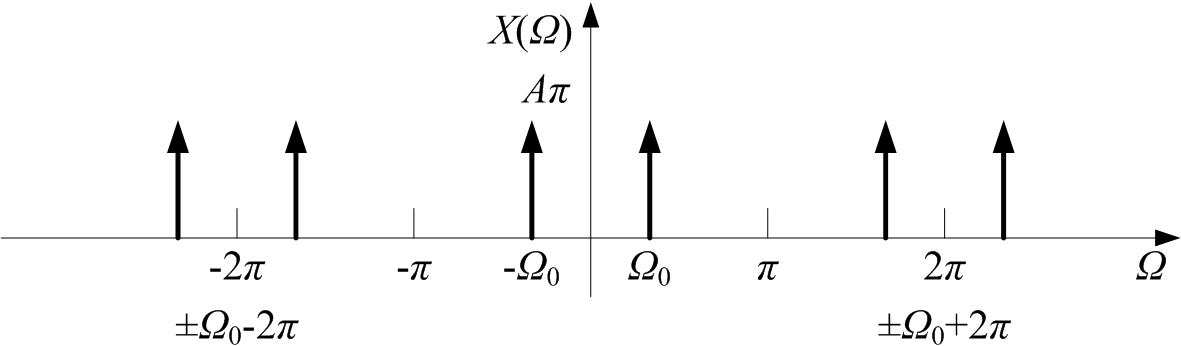
\includegraphics[height=3cm]{6.2.2-2.png}
\end{figure}

再考察采样对输出的影响。
假设连续时域信号$x\left( t \right) =A\cos \left( \omega _0t \right) $,对其采样
\begin{align*}
&x\left[ n \right] =\left. x\left( t \right) \right|_{t=nT}=A\cos \left( \omega _0nT \right) \overset{\varOmega _0=\omega _0T}{=}A\cos \left( \varOmega _0n \right) \\
&n=0,\pm 1,\pm 2,\cdots
\end{align*}
要使$\varOmega _0\leqslant B$,即$\omega _0T\leqslant B$,也即$T\leqslant B/\omega _0$。

\begin{tcolorbox}
采样频率越高,DTFT映射到的实际频率范围越宽。
\end{tcolorbox}

%============================================================
\subsection{均值滤波器}

考虑最简单的平均化,系统的输入输出差分方程为:
\[
y\left[ n \right] =\frac{1}{N}\sum_{k=0}^{N-1}{x\left[ n-k \right]}
\]
一般认为当$N\geqslant 3$时有较为锋利的截止,这样的系统称为{\bf 均值滤波器}(mean filter),频率响应函数:
\begin{align*}
&\because h\left[ n \right] =\frac{1}{N}\sum_{k=0}^{N-1}{\delta \left[ n-k \right]} \\
&\because \begin{cases}
	x\left[ n-n_1 \right] \leftrightarrow X\left( \varOmega \right) \cdot e^{-i\varOmega n_1}\\
	\delta \left[ n \right] \leftrightarrow 1\\
\end{cases} \\
&\therefore H\left( \varOmega \right) =\frac{1}{N}\sum_{k=0}^{N-1}{e^{-i\varOmega k}}
\end{align*}

\begin{python}
def mean_filter(N, W):
	H = 1
	for i in range(1, N):
		H = H + np.exp(-1.0j * i * W)
		pass
	H = H / N
	return H

W  = np.arange(-3*np.pi, 3*np.pi, 0.01)
N1 = 2;  H1 = mean_filter(N1, W)
N2 = 5 ; H2 = mean_filter(N2, W)
N3 = 20; H3 = mean_filter(N3, W)

plot_mag_phs(W, np.abs(H1), np.angle(H1, deg=True), ...)
plot_mag_phs(W, np.abs(H2), np.angle(H2, deg=True), ...)
plot_mag_phs(W, np.abs(H3), np.angle(H3, deg=True), ...)
\end{python}

\begin{figure}[h]
\centering
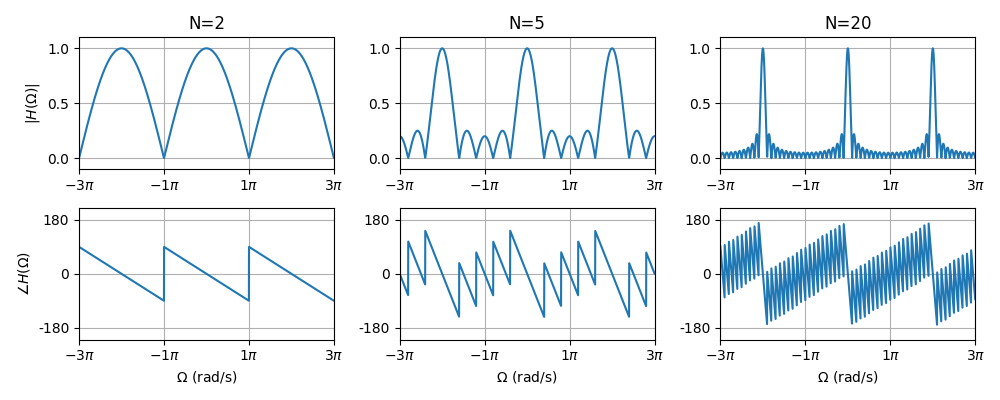
\includegraphics[height=4cm]{6.2.3-1.png}
\end{figure}

由幅频图可得系统是个低通,且阶数越高带宽越小,时域上就是抹得越平。




